\subsection{Noise}

\begin{figure}[t!]
  \centering
  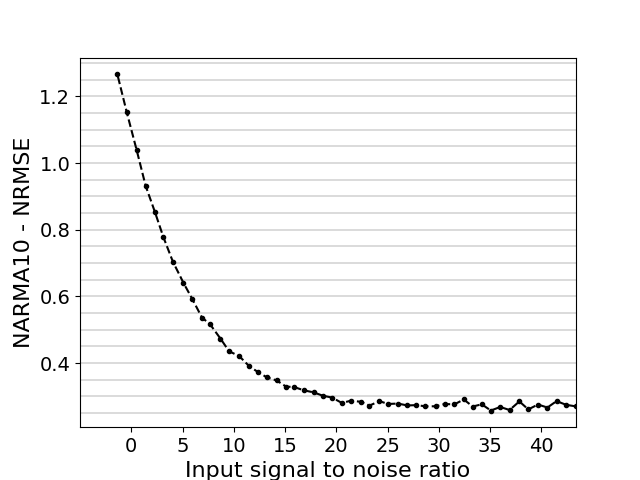
\includegraphics[width=3.3in]{img/input_noise_snr.png}
  \caption{
    Noise causing a decrease in performance for an ESN reservoir on the NARMA10
task. When the signal to noise ratio drops below 20dB, the performance of the
reservoir degrades in an exponential manner.
  }
  \label{input_noise_snr}
\end{figure}

In this experiment we vary the input signal to noise ratio. The results are
shown in Fig. \ref{input_noise_snr}, illustrating an increase in error when the
ratio of signal power to noise power drops below 20 dB. The reservoir error
increases more drastically below 10 dB, quickly becoming insufficient for the
prediction task. A similar increase in error has been seen in previous work,
using the same SNR measure to evaluate signal reconstruction capacity in a
dynamical system \cite{dambre_information_2012}.

The eventual diminishing return from increasing the signal to noise ratio seen
in Fig. \ref{input_noise_snr} is expected given the relationship between
information transmission capacity and SNR given by the Shannon-Hartley
theorem. This is related to our results in the sense that we can compare the
information processing capabilities of a reservoir in the presence of noise with
that of already established communications. For example, commonly recommended
SNRs in the IEEE 802.11 standard for Wi-Fi communications range from 15db to
25dB when using standardized bandwidth bands of 2.4GHz and 5GHz. Hence, maximum
theoretical channel capacities are determined by the $\frac{S}{N}$ term, in
which the signal is determined by power radiation from the antenna, and the
noise by equipment quality and interference. Below the given threshold, wireless
communication will quickly become unusable.

\subsection{Measurement equipment accuracy}

\begin{figure}[t!]
  \centering
  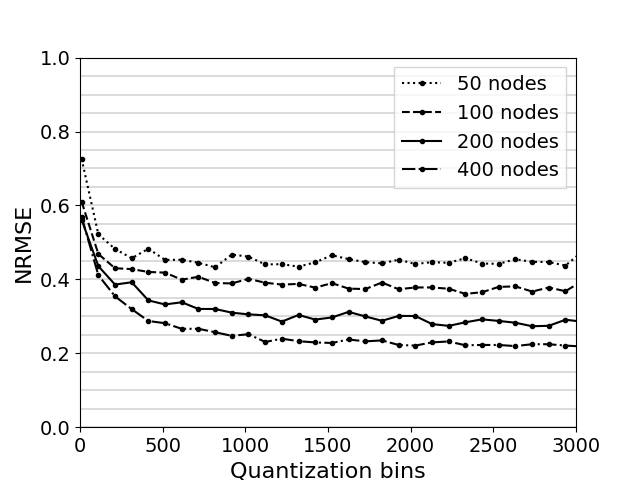
\includegraphics[width=3.3in]{img/adc_quantization.png}
  \caption{
    Performance effect of ADC quantization on four reservoirs of different
sizes. The range (-1, 1) of the $\tanh$ activation function is divided into
$2^n$ discrete output bins.
  }
  \label{adc_quantization}
\end{figure}

We extend the ESN model to quantize the activation of the internal nodes of the
reservoir. Fig. \ref{adc_quantization} shows a performance degradation from 12
to 10 quantization bits. As discrete output states move beneath a quantization
of 10 bits, the performance quickly deteriorates. However, even with just 4 bits
to discretely separate outputs, reservoirs are still able to replicate the input
sequence to some degree. Furthermore, reservoirs with 400 hidden nodes and just
64 output bins consistently provide the same performance as that of a reservoir
with 50 hidden nodes and no output quantization.

A 12-bit ADC has $2^{12}$, or 4096 output codes, which in accordance with our
experiments would impose little increase in the prediction error. 16-bit ADCs,
outputting $2^{16}$, or 65536 discrete states, would influence our ESN
simulations even less.

Previously, a major factor limiting the performance of a nonlinear analog
electric circuit implementation has been found to be quantization noise
\cite{soriano_delay-based_2015}. Low error rates on the Mackey-Glass task were
achieved with 8 bits or more in the ADC. This result differs from the
performance measures seen in our ESN implementation, where NRMSE starts leveling
out around 10 bits of accuracy.

We attribute this discrepancy to the nature of the $\tanh$ activation. In our
experiment, $\tanh$ is divided linearly into discrete bins, although we may not
use the complete range. As the NARMA10 task relies heavily upon memory, and less
so upon nonlinearity, the activation of a high number of nodes will lie in the
highly linear part of $\tanh$ in the interval [-0.4, 0.4], with a few nodes
outside this range. Essentially, this may in the worst cases account for halving
the available output bins

\subsection{Partially observable reservoir state}

\begin{figure*}[t!]
  \centering
  \begin{subfigure}{.49\textwidth}
    \centering
    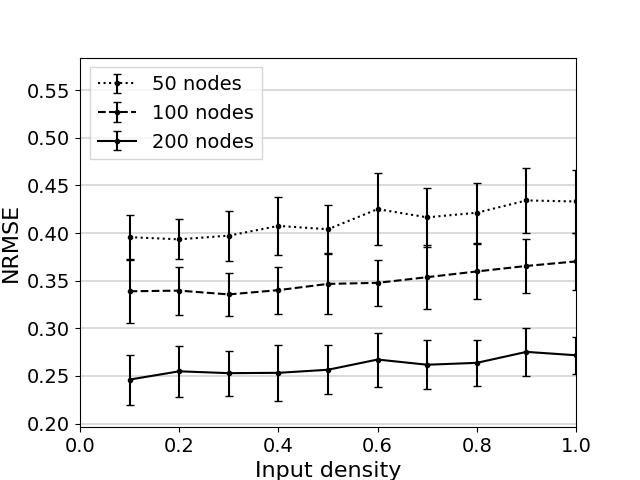
\includegraphics[width=1.0\linewidth]{img/input_density_all.png}
    \caption{}
  \end{subfigure}
  \begin{subfigure}{.49\textwidth}
    \centering
    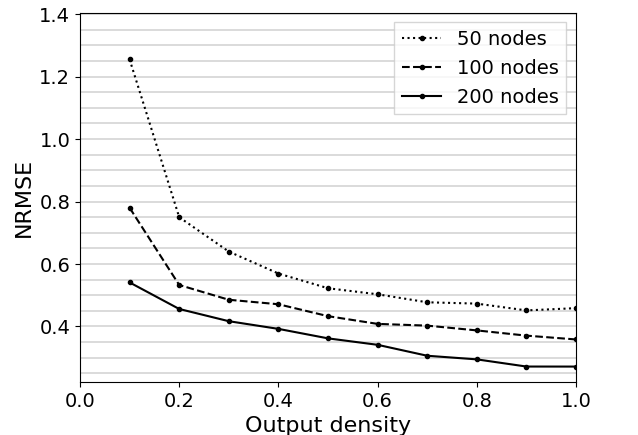
\includegraphics[width=1.0\linewidth]{img/output_density_all.png}
    \caption{}
  \end{subfigure}
  \caption{
    Influence of reservoirs that are only partially visible on the
performance. The density is a measurement for the fraction of elements in the
input and output matrices containing non-zero elements.
  }
  \label{partial_visibility}
\end{figure*}

First, we investigate partially visible reservoirs by adjusting the sparsity of
$\mathbf{W}_{in}$. Results are shown in Fig. \ref{partial_visibility}a, in which
all experiments were done with a uniform input weight distribution in the
interval [-0.5, 0.5].

Across all three reservoir sizes, we see a small increase in the signal
prediction error when increasing input connectivity from an initial density of
0.1. While finding the optimal reservoir perturbance clearly depends on the
memory capacity and computational dynamics required for the task at hand, this
benchmark task gives a clear indication of the influence of input sparsity in
general. The relatively low sensitivity to this parameter suggests that physical
reservoirs may achieve excellent performance even when only perturbing selected
parts of the system. An input stream parameter found to be of greater relevance
is input scaling, i.e. the amplitude of the input signal that the reservoir sees
\cite{alippi_quantification_2009}. The necessary scaling depends on the
nonlinearity needed, as inputs far from 0 drive $\tanh$ neurons towards
saturation. In a physical reservoir design setting, this parameter is often
possible to adjust after-the-fact, as opposed to changing the physical hardware
layout of the system.

Next, a general trend seen when adjusting output connectivity, is a slight,
linear decrease in performance from a completely dense output matrix to a
density of 0.4 (Fig. \ref{partial_visibility}b). Furthermore, for the 50 and 100
node reservoirs, there is a noticeable transition from a linear to an
exponential NRMSE growth.

We may understand these results to indicate that there is a critical point in
the output density space where the readout layer starts seeing enough of the
reservoir dynamics to reconstruct the input NARMA10 signal. Additionally, when
the output density exceeds this threshold, the performance will continue to grow
linearly with the density, achieving the best performance at full connectivity.

Another interesting result illustrated in Fig. \ref{partial_visibility}b is that
increasing the reservoir size without increasing the amount of output nodes has
little effect on the network performance. Changing the x-axis of the previous
plot to the actual amount of connected nodes instead of the output density
reveals this conclusively, as seen in Fig. \ref{output_nodes}.

\begin{figure}[t!]
  \centering
  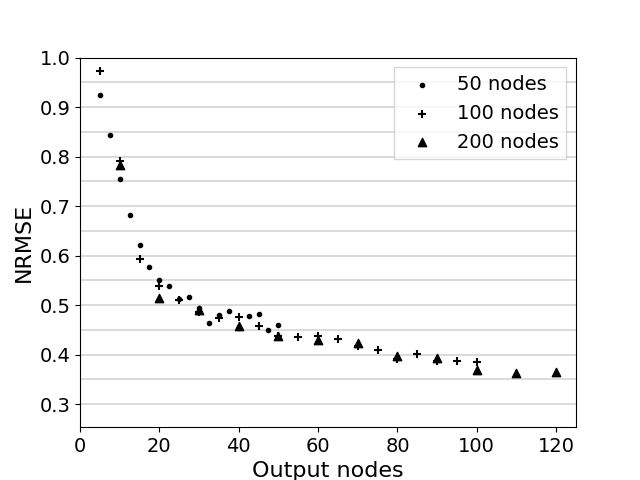
\includegraphics[width=3.3in]{img/output_nodes.png}
  \caption{
    Performance of reservoirs of three different sizes, as a function of the
amount of reservoir nodes connected to the readout layer. There is no clear
distinction between the reservoir sizes, demonstrating that increasing reservoir
sizes have no effect on performance if the output sampling remains the same.
  }
  \label{output_nodes}
\end{figure}

Our results suggest that in the case of output connectivity, the performance of
reservoir systems only correlates with the absolute amount of nodes seen, and
not with the internal reservoir size. Hence, physical reservoir implementations
must carefully consider this property, making it imperative that a partial
visibility of the reservoir dynamics is sufficient for the task of which it is
designed. In essence, the gathered information that is present in clusters of
neurons on microelectrode grids may be completely lost if the layout is too
sparse.

% (TODO): Discuss how this relates to the maximum information capacity of
% individual nodes, and include Shannon information and how complexity is defined
% as the amount of information required to describe something.

\begin{figure}[t!]
  \centering
  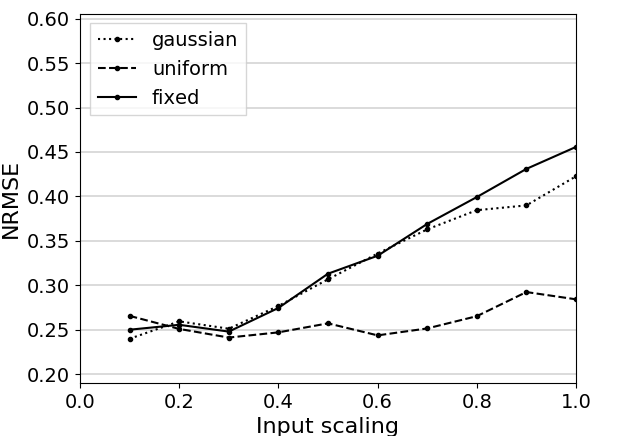
\includegraphics[width=3.3in]{img/input_scaling_distrib.png}
  \caption{
    Effect of input scaling on three input weight distributions. With the fixed
distribution every input weight is set to 1. The best performance of all three
distributions lie around NRMSE $\approx 0.25$.
  }
  \label{input_scaling_distrib}
\end{figure}

It is well-established in RC methodology that using a uniform distribution of
input weights in some interval [-a, a] gives good performance. However, is it
possible to achieve a competitive error rate using other weight distributions?
Fig. \ref{input_scaling_distrib} explores the performance of ESNs with three
different input weight distributions: uniform, Gaussian and fixed. Despite the
performance disparity with increasing input scaling, the best performance of all
three classes hover around the same NRMSE of around 0.25. This demonstration of
scaling differently distributed inputs such that they all achieve acceptable
performance bodes well for physical RC. In particular, we observe a promising
result when considering RC with physical substrates in which every node is
forced to receive the same input. Exploring different $\mathbf{W}_{in}$
distributions in ESNs may give an intuition for its importance as a reservoir
parameter, which may provide valuable in reservoir design, as one may resort to
the simplest or cheapest solution.

%%% Local Variables:
%%% mode: latex
%%% TeX-master: "../main"
%%% End:
